% --------------------------------------------------
\section*{Résumé}
% --------------------------------------------------

Les interfaces web modernes exigent des capacités de communication temps réel de plus en plus performantes. Le choix du protocole de communication entre le serveur et le client est une décision technique critique qui impacte directement les performances, la maintenabilité du code et la qualité de l'expérience utilisateur. Si WebSocket et Server-Sent Events sont aujourd'hui des technologies matures et bien documentées, WebTransport propose une alternative potentiellement plus performante, mais encore peu étudiée dans le contexte des interfaces web développées avec des frameworks modernes comme Angular. Ce travail propose une étude expérimentale comparative de ces trois protocoles appliqués à un dashboard Angular temps réel, en mesurant la latence, la résilience aux conditions réseau dégradées et la complexité d'intégration. L'objectif est de fournir des éléments concrets et mesurés permettant aux développeurs d'interfaces web de choisir le protocole le mieux adapté à leur contexte applicatif.

% --------------------------------------------------
\section{Introduction}
% --------------------------------------------------

\subsection{Contexte}

Le développement des applications web a connu une mutation au cours des deux dernières décennies. Là où le web reposait initialement sur un modèle requête-réponse --- le client demande, le serveur répond --- aujourd'hui, les applications web ne se contentent plus d'afficher des pages statiques. Les utilisateurs s'attendent à voir les données se mettre à jour en direct, sans avoir à recharger la page. C'est le cas par exemple d'un tableau de bord, d'un outil de monitoring ou encore d'une interface financière affichant des cours en temps réel, sans intervention de l'utilisateur.

Pour répondre à ce besoin, plusieurs protocoles de communication temps réel ont été créés, chacun répondant à des contraintes techniques et des usages différents. Parmi eux, WebSocket, standardisé en 2011, est aujourd'hui le plus répandu : il ouvre une connexion persistante et bidirectionnelle entre le client et le serveur. Server-Sent Events (SSE) est une alternative plus simple, qui repose sur HTTP classique et permet au serveur d'envoyer des données au client de façon continue, mais dans un seul sens (unidirectionnel). Enfin, WebTransport est un protocole beaucoup plus récent, basé sur QUIC et HTTP/3, qui promet de meilleures performances réseau et de réduire la latence, mais qui reste encore peu adopté et peu documenté dans la pratique.

Dans ce contexte, un développeur d'IHM web fait face à plusieurs interrogations : lequel choisir ? Pour quel cas d'usage ? Avec quels compromis ? Cette décision concerne les performances techniques du système, mais aussi la qualité de l'expérience utilisateur finale et la maintenabilité du code qui est produit.

\subsection{Motivation}

Ce sujet de recherche a principalement été choisi car il permettait de combiner deux domaines de l'informatique qui m'intéressent le plus : les réseaux et le développement web. Académiquement, les réseaux sont l'une des matières qui m'intéressent le plus et vers lesquelles j'hésite à m'orienter après mes études. En parallèle, ma mission d'apprentissage en entreprise est le développement d'interfaces Homme-Machine web avec le framework Angular. J'ai notamment eu l'occasion de commencer le développement d'un dashboard de monitoring. Ce sujet était donc une manière de relier ces deux aspects en explorant comment les protocoles réseau influencent concrètement ce que l'on développe côté front-end.

Si WebSocket et SSE sont des technologies plutôt connues et bien documentées, WebTransport reste à l'inverse une technologie très récente et encore peu étudiée dans le contexte des frameworks frontend modernes. Il repose sur QUIC, un protocole de transport récent qui sert également de base à HTTP/3. QUIC avait d'ailleurs été brièvement évoqué dans mon cours de réseaux, ce qui m'avait rendue curieuse. Peu d'études expérimentales comparent WebTransport aux deux autres protocoles, surtout dans un contexte d'IHM Angular, ce qui rend ce projet d'autant plus intéressant à étudier.

\subsection{Objectifs}

Ce projet de recherche a trois objectifs principaux :

\begin{itemize}
    \item Comparer les performances des trois protocoles dans des conditions expérimentales équitables, en se concentrant sur des fonctionnalités communes aux trois technologies.
    \item Mesurer leur impact sur l'expérience utilisateur via des métriques quantitatives comme la latence et le comportement sous charge.
    \item Évaluer la complexité d'intégration de chaque protocole dans un projet Angular avec un backend Node.js.
\end{itemize}

% --------------------------------------------------
\section{Problématique}
% --------------------------------------------------

Les trois protocoles étudiés permettent tous de faire la même chose de base : envoyer des données depuis un serveur vers un client web en temps réel. Cependant, leurs architectures techniques et leurs comportements dans des conditions réseau variées diffèrent.

\begin{center}
\textit{Dans quelle mesure le choix du protocole de communication temps réel influence-t-il les performances et l'expérience utilisateur d'un dashboard Angular, et quel protocole offre le meilleur compromis entre latence, résilience et complexité d'intégration ?}
\end{center}

Cette problématique se décline en trois sous-questions qui guideront les expérimentations :

\begin{enumerate}
    \item \textbf{Performance :} Quelles différences de latence et de débit mesure-t-on entre WebSocket, SSE et WebTransport dans des conditions réseau normales et sous charge ? La latence est calculée via un timestamp envoyé dans chaque message, et le débit correspond au nombre de messages effectivement reçus par seconde.
    \item \textbf{Résilience :} Comment chaque protocole réagit-il face à une coupure réseau simulée, et quel est l'impact visible sur l'interface ? On mesure le temps de reconnexion de chaque protocole après interruption.
    \item \textbf{Intégration :} Quelle est la complexité relative de la mise en place de chaque protocole dans une architecture Angular + Node.js ?
\end{enumerate}

L'idée est de pouvoir, à l'issue des expérimentations, donner des recommandations pratiques à destination d'un développeur web qui se poserait les mêmes questions que moi.

% --------------------------------------------------
\section{État de l'art}
% --------------------------------------------------

\subsection{Les besoins des IHM web temps réel}

Avant de présenter les protocoles, il est important de comprendre pourquoi le temps réel est devenu un enjeu central dans le développement d'interfaces web. De nos jours, un utilisateur qui consulte un dashboard de monitoring s'attend à ce que les données se mettent à jour automatiquement sans avoir à rafraîchir la page. Si l'interface met plusieurs secondes à refléter un changement, ou pire, si elle se fige lors d'une instabilité réseau, l'expérience utilisateur est directement touchée négativement.

On distingue généralement deux grands types de besoins dans ce contexte :

\begin{itemize}
    \item \textbf{Le push serveur :} le serveur envoie des données au client sans que celui-ci en fasse la demande explicitement. C'est le cas typique d'un dashboard qui affiche des métriques mises à jour automatiquement.
    \item \textbf{La communication bidirectionnelle :} le client et le serveur échangent des données dans les deux sens simultanément, comme dans une application de chat ou un jeu en ligne.
\end{itemize}

Dans le cadre de ce projet, on se concentre sur le push serveur, car c'est la fonctionnalité commune aux trois protocoles étudiés, ce qui permet une comparaison équitable.

\subsection{WebSocket}

WebSocket est un protocole de communication standardisé par l'IETF en 2011 (RFC 6455). Il fonctionne comme une « ligne téléphonique » entre le client et le serveur : une fois la connexion établie, les deux parties peuvent s'échanger des messages librement et simultanément, sans avoir à rouvrir une connexion à chaque échange. WebSocket repose sur une connexion TCP persistante établie grâce à un mécanisme d'upgrade HTTP : le client envoie une requête HTTP classique avec un en-tête \texttt{Upgrade: websocket}, et si le serveur accepte, la connexion bascule vers WebSocket.

WebSocket est aujourd'hui la technologie la plus mature et la plus utilisée pour le temps réel web. Son support navigateur est universel, sa documentation abondante, et les bibliothèques disponibles dans tous les langages et frameworks sont nombreuses. C'est le choix par défaut de la grande majorité des applications temps réel en production.

Cependant, sa nature bidirectionnelle introduit une complexité inutile lorsqu'on n'a besoin que d'un flux de données dans un seul sens. De plus, WebSocket repose sur TCP, signifiant qu'en cas de perte de paquets, l'ensemble du flux est bloqué en attendant la retransmission. C'est un phénomène connu sous le nom de \textit{head-of-line blocking}. Enfin, WebSocket ne gère pas la reconnexion automatique nativement : c'est au développeur de l'implémenter.

\subsection{Server-Sent Events (SSE)}

Server-Sent Events est une technologie standardisée (initialement par le W3C, et désormais maintenue dans le \textit{HTML Living Standard} du WHATWG) qui permet à un serveur d'envoyer des données en continu vers un client via une connexion HTTP longue durée. Contrairement à WebSocket, SSE est strictement unidirectionnel : seul le serveur envoie des données. Les événements sont transmis sous forme de texte dans un format simple :

\begin{lstlisting}
event: message
data: {"valeur": 42}
id: 1
\end{lstlisting}

SSE est remarquablement simple à mettre en place. Il repose sur HTTP standard sans nécessiter d'upgrade de protocole ; il est donc compatible avec les infrastructures existantes sans configuration particulière. Il gère également la reconnexion automatique nativement : si la connexion est perdue, le navigateur tente automatiquement de se reconnecter, ce qui simplifie beaucoup la gestion des erreurs côté client. Enfin, il fonctionne très bien avec HTTP/2 et son multiplexage, ce qui le rend efficace pour des flux en lecture seule.

Sa principale limitation est son caractère strictement unidirectionnel. Le client ne peut pas envoyer de données via SSE et doit passer par des requêtes HTTP séparées pour communiquer avec le serveur. Il est donc inadapté dans des cas d'usage nécessitant des échanges dans les deux sens. Par ailleurs, SSE ne supporte que le texte (pas de données binaires), et les navigateurs imposent une limite sur le nombre de connexions SSE simultanées par domaine. Enfin, comme WebSocket, SSE repose sur TCP et est donc sujet au même problème de \textit{head-of-line blocking}.

\subsection{WebTransport}

WebTransport est un protocole récent actuellement en cours de standardisation par le W3C et l'IETF. Il repose sur QUIC, un protocole de transport développé initialement par Google et standardisé en 2021 (RFC 9000), qui constitue également la base de HTTP/3 --- la troisième version du protocole web, conçue pour résoudre les limitations de HTTP/2 en abandonnant TCP pour QUIC. Contrairement à TCP, QUIC fonctionne sur UDP et intègre nativement le chiffrement TLS 1.3, ce qui signifie que la sécurisation des données est établie en même temps que la connexion, sans étape supplémentaire. Le temps de connexion initial est donc réduit par rapport aux protocoles précédents.

WebTransport propose deux modes de communication : les \textit{streams fiables} (avec garantie de livraison et d'ordre, similaires à TCP) et les \textit{datagrams non fiables} (sans garantie mais avec latence minimale, similaires à UDP). Cette flexibilité est l'une de ses principales innovations.

Grâce à QUIC, WebTransport résout le problème de \textit{head-of-line blocking} présent dans WebSocket et SSE. En cas de perte d'un paquet sur un flux, les autres flux ne sont pas bloqués. De plus, QUIC permet une meilleure gestion des changements de réseau, par exemple lors d'un passage du Wi-Fi à la 4G sans interruption de session. WebTransport supporte également le multiplexage natif de plusieurs flux indépendants sur une seule connexion : au lieu d'envoyer les données les unes après les autres, plusieurs flux peuvent transiter en parallèle et de façon indépendante. Si un flux rencontre un problème réseau (perte de paquet par exemple), les autres ne sont pas bloqués, ce qui réduit la latence globale perçue. Enfin, WebTransport supporte également la communication bidirectionnelle, ce qui en fait une alternative potentiellement plus performante à WebSocket.

Cependant, WebTransport est encore très jeune. Son support navigateur reste limité principalement à Chrome et Edge, Firefox étant en cours d'implémentation. La configuration d'un serveur WebTransport est plus complexe que pour WebSocket ou SSE et nécessite obligatoirement HTTPS avec un certificat valide. Très peu de projets en production l'utilisent à ce jour ; le retour d'expérience pratique reste donc encore plutôt rare.

\subsection{Synthèse comparative}

\begin{table}[H]
\centering
\small
\begin{tabular}{|l|c|c|c|}
\hline
\textbf{Critère} & \textbf{WebSocket} & \textbf{SSE} & \textbf{WebTransport} \\
\hline
Standard & RFC 6455 (2011) & W3C (2006) & W3C/IETF (en cours) \\
Protocole de base & TCP & HTTP/TCP & QUIC/UDP \\
Direction & Bidirectionnel & Unidirectionnel & Bidirectionnel \\
Head-of-line blocking & Oui & Oui & Non \\
Reconnexion auto & Non (à gérer) & Oui (native) & Non (à gérer) \\
Support navigateur & Universel & Universel & Partiel (Chrome/Edge) \\
Données binaires & Oui & Non & Oui \\
Maturité & Très élevée & Élevée & Faible \\
Complexité mise en place & Moyenne & Faible & Élevée \\
\hline
\end{tabular}
\caption{Synthèse comparative des trois protocoles}
\end{table}

\begin{table}[H]
\centering
\small
\begin{tabular}{|l|l|p{2.1cm}|p{2.8cm}|p{2.8cm}|}
\hline
\textbf{Technologie} & \textbf{Type} & \textbf{Transport} & \textbf{Points forts} & \textbf{Cas d'usage} \\
\hline
SSE & Unidirectionnel & HTTP/1.1 ou HTTP/2 & Léger, reconnexion auto, simple & Flux de prix, notifications \\
\hline
WebSocket & Bidirectionnel & TCP (upgrade HTTP) & Très compatible, full-duplex & Chats, outils collaboratifs \\
\hline
WebTransport & Bidirectionnel & HTTP/3 (QUIC) & Ultra-basse latence, supporte l'instantanéité (datagrammes) & Gaming, streaming vidéo HD, IoT \\
\hline
\end{tabular}
\caption{Synthèse par type, transport et cas d'usage}
\end{table}

Cette synthèse montre que chaque protocole répond à des besoins différents. WebSocket reste la valeur sûre et universelle, SSE est idéal pour les cas simples de push serveur, et WebTransport représente une piste prometteuse pour les applications nécessitant de très faibles latences. C'est précisément ce que les expérimentations de ce projet cherchent à quantifier concrètement à l'aide du développement d'un dashboard Angular.

% --------------------------------------------------
\section{Méthodologie}
% --------------------------------------------------

\subsection{Architecture du banc de test}

Dans le but de comparer les trois protocoles de façon équitable, j'ai développé une application de test composée de deux parties : un backend Node.js déployant trois serveurs, un par protocole, et un frontend Angular affichant un dashboard temps réel commun.

Le principe est simple : les trois serveurs envoient exactement les mêmes données, au même moment et dans le même format JSON. Seul le protocole de transport est différent. Le dashboard reçoit ensuite les données, calcule les métriques en temps réel et les affiche sous forme de graphiques en barres.

\begin{table}[H]
\centering
\small
\begin{tabular}{|l|l|l|}
\hline
\textbf{Composant} & \textbf{Rôle} & \textbf{Port / URL} \\
\hline
websocket-server.js & Push WebSocket & ws://localhost:3001 \\
sse-server.js & Push SSE (Express) & http://localhost:3002/events \\
webtransport-server.js & Push WebTransport & https://\textless{}hôte\textgreater{}:3003/webtransport \\
Dashboard Angular & Mesure, visualisation, export CSV & http://\textless{}hôte\textgreater{}:4200 \\
\hline
\end{tabular}
\caption{Composants du banc de test}
\end{table}

\textbf{Environnement technique :}

\begin{itemize}
    \sloppy
    \item Backend : Node.js v24, bibliothèques \texttt{ws} (WebSocket), Express + CORS (SSE), \texttt{@fails-components/}\allowbreak\texttt{webtransport} (WebTransport)
    \item Frontend : Angular 17+ exécuté dans Google Chrome
    \item Machine de test : machine unique sous Linux (WSL2), le navigateur Google Chrome tournant sous Windows. WebSocket et SSE ont été testés via \texttt{localhost}, tandis que WebTransport et certaines mesures de l'expérience 3 nécessitaient de passer par l'IP LAN du poste (ex. \texttt{http://192.168.1.194:4200}), en raison des contraintes TLS et de la configuration réseau propre à WSL2.
    \item Simulation réseau dégradé : script iptables bloquant complètement le trafic sur les ports des trois serveurs pendant 5 secondes.
\end{itemize}

Le choix de Google Chrome s'impose par nécessité technique : WebTransport n'est pas encore supporté par tous les navigateurs. Firefox, par exemple, ne le supporte pas encore pleinement. Ce choix est lui-même une observation expérimentale sur la maturité de WebTransport.

\subsection{Définition des métriques}

Pour que la comparaison soit scientifiquement valide, les métriques choisies s'appliquent aux trois protocoles de la même façon et ne favorisent par nature aucun d'entre eux. On s'est concentré uniquement sur le push serveur (l'envoi de données du serveur vers le client), qui constitue la seule fonctionnalité réellement commune aux trois protocoles. Par exemple, tester la communication bidirectionnelle aurait favorisé WebSocket et WebTransport, au détriment de SSE qui ne la supporte pas nativement.

\begin{itemize}
    \item \textbf{Métrique 1 --- Latence bout-en-bout :} temps qui s'écoule entre le moment où le serveur envoie un message et le moment où l'interface l'affiche. Chaque message contient un champ \texttt{timestamp} indiquant l'heure d'émission en millisecondes. Le client calcule la différence avec l'heure actuelle via \texttt{Date.now()}. C'est la métrique la plus directement liée à l'expérience utilisateur. Il faut toutefois noter que \texttt{Date.now()} a une résolution de l'ordre de la milliseconde : une mesure individuelle vaut donc 0, 1 ou 2 ms entiers, et les latences moyennes inférieures à 1 ms rapportées plus loin traduisent une \textit{tendance} plutôt qu'un classement strict entre protocoles.

    \item \textbf{Métrique 2 --- Débit (Throughput) :} nombre de messages réellement reçus par le client chaque seconde. Cette métrique complète la latence en révélant si un protocole perd des messages quand la fréquence d'envoi augmente. Elle est calculée côté client en comptant les messages reçus sur des fenêtres d'une seconde.

    \item \textbf{Métrique 3 --- Résilience :} comportement de chaque protocole lors d'une interruption réseau. On mesure le temps entre la coupure et le retour des données dans l'interface, ainsi que le comportement visible dans le dashboard (interface qui fige ou non, reconnexion automatique ou non, perte de données).

    \item \textbf{Métrique 4 --- Complexité d'intégration :} métrique qualitative évaluant la difficulté de mise en place de chaque protocole. On compare le nombre de lignes de code nécessaires côté serveur et côté client, les dépendances à installer et les difficultés rencontrées lors de la configuration.
\end{itemize}

\textbf{Note sur le temps de traitement :} une métrique de temps de traitement des messages côté client avait été envisagée via \texttt{performance.now()}. Elle a été abandonnée car les navigateurs limitent volontairement la précision de cette API à 1~ms pour des raisons de sécurité. Parser un petit objet JSON prend moins de 0,1~ms, ce qui est en dessous de ce seuil et rend la mesure inexploitable. Cela confirme que le temps de traitement côté client n'est pas le facteur limitant : c'est bien le transport réseau qui fait la différence entre les protocoles.

\subsection{Protocole expérimental}

\textbf{Expérience 1 --- Latence en conditions normales.} \textit{Objectif} : établir une baseline de performance pour chaque protocole dans des conditions réseau idéales. \textit{Déroulement} : le serveur envoie 1 message par seconde contenant un timestamp et une valeur numérique simulée. Les trois protocoles sont connectés simultanément. On laisse tourner 2 minutes puis on exporte les données en CSV. \textit{Métriques relevées} : latence moyenne, minimale et maximale pour chaque protocole.

\textbf{Expérience 2 --- Latence sous charge croissante.} \textit{Objectif} : observer comment la latence évolue lorsque la fréquence d'envoi augmente, et identifier à partir de quel seuil les protocoles commencent à se différencier. \textit{Déroulement} : on fait varier la fréquence d'envoi : 1, 10, 50 et 100 messages par seconde. Pour chaque fréquence, on mesure la latence moyenne et le débit sur 1 minute, puis on exporte le CSV. \textit{Métriques relevées} : latence moyenne et débit par fréquence et par protocole.

\textbf{Expérience 3 --- Résilience face à une coupure réseau.} \textit{Objectif} : comparer le comportement de chaque protocole lors d'une interruption réseau et mesurer son impact sur l'interface utilisateur. \textit{Déroulement} : on établit une connexion stable à 1 message par seconde pour les trois protocoles. On simule ensuite une coupure réseau de 5 secondes via un script iptables --- un outil Linux de filtrage réseau --- qui bloque complètement le trafic entrant et sortant sur les ports des trois serveurs (3001, 3002 et 3003). Il s'agit donc d'une coupure totale des ports du banc de test, et non d'une simple perte de paquets. L'expérience est répétée 3 fois. \textit{Métriques relevées} : temps de reconnexion, comportement UI pendant la coupure.

\textbf{Expérience 4 --- Complexité d'intégration.} \textit{Objectif} : évaluer le coût de développement associé à chaque protocole, au-delà des seules performances techniques. \textit{Déroulement} : on compare les implémentations des trois protocoles côté serveur (Node.js) et côté client (Angular) en comptant les lignes de code nécessaires, en recensant les dépendances requises et en documentant les difficultés rencontrées lors de la mise en place. \textit{Métriques relevées} : lignes de code côté serveur et côté client, nombre de dépendances, difficultés de configuration.

\subsection{Précautions pour garantir l'équité des mesures}

Le risque principal dans ce type de comparaison est de concevoir des expériences qui favorisent par nature l'un des protocoles. Pour l'éviter, les précautions suivantes ont été prises :

\begin{itemize}
    \item Même format de données pour les trois protocoles (JSON texte uniquement), y compris pour WebSocket qui supporte le binaire, afin d'être équitable avec SSE.
    \item Même fréquence d'envoi pour les trois protocoles lors de chaque expérience.
    \item Même navigateur (Google Chrome) pour les trois protocoles.
    \item Fonctionnalité commune testée : uniquement le push serveur, pas la bidirectionnalité qui avantagerait naturellement WebSocket et WebTransport.
    \item Même machine pour tous les tests, afin d'éliminer les variations matérielles.
\end{itemize}

% --------------------------------------------------
\section{Résultats}
% --------------------------------------------------

\subsection{Expérience 1 --- Latence en conditions normales}

Cette première expérience a été menée sur une durée d'environ 2 minutes avec l'envoi d'un message par seconde, les trois protocoles étant connectés simultanément depuis le dashboard Angular. Au total, 137 messages ont été reçus par protocole, ce qui confirme que le débit cible a bien été atteint ($\sim$1,01 msg/s pour les trois).

\begin{table}[H]
\centering
\begin{tabular}{|l|c|c|c|c|}
\hline
\textbf{Protocole} & \textbf{n} & \textbf{Latence moy. (ms)} & \textbf{Min (ms)} & \textbf{Max (ms)} \\
\hline
WebSocket & 137 & 0,08 & 0 & 2 \\
SSE & 137 & 0,37 & 0 & 3 \\
WebTransport & 137 & 0,63 & 0 & 43 \\
\hline
\end{tabular}
\caption{Résultats expérience 1 --- latence à 1 msg/s}
\end{table}

WebSocket présente la latence moyenne la plus faible (0,08 ms), suivi de SSE (0,37 ms) puis WebTransport (0,63 ms). Ces trois valeurs restent très faibles (en dessous de 1 ms) et les écarts entre elles sont modestes dans des conditions locales idéales. Pour rappel, la latence mesurée ici correspond au temps écoulé entre le moment où le serveur envoie un message et le moment où Angular l'affiche dans le dashboard.

WebTransport se distingue par un pic de latence isolé à 43 ms, visible sur les outliers du graphique de la figure~\ref{fig:exp1}. Ce pic correspond au temps d'établissement de la connexion QUIC lors du premier message. Il nécessite une phase d'initialisation plus longue que TCP lors de la première connexion. Ce comportement disparaît ensuite et ne se reproduit pas sur les messages suivants. L'histogramme confirme que la quasi-totalité des messages WebTransport se situent dans la tranche 0--1 ms, au même niveau que les deux autres protocoles.

\begin{figure}[H]
\centering

\includegraphics[width=\textwidth]{articles/fig/exp1_latence.pdf}
\caption{Expérience 1 --- latence à 1 msg/s en conditions locales. De gauche à droite : zoom 0--6 ms, répartition par tranche, synthèse médiane/moyenne/P95, outliers > 5 ms.}
\label{fig:exp1}
\end{figure}

Visuellement dans le dashboard, les barres WebSocket restent très plates avec de rares pics ponctuels, SSE affiche un profil légèrement plus irrégulier avec de petites variations fréquentes, et WebTransport montre des pics isolés visuellement marquants malgré une médiane similaire aux deux autres protocoles.

\paragraph{Expérience 1b --- latence simulée (\texttt{tc netem}).}
À titre complémentaire, une latence artificielle de 50 ms (avec une variation de 10 ms) a été injectée sur la connexion locale à l'aide de \texttt{tc netem delay 50ms 10ms sur lo}, un outil Linux permettant de simuler des conditions réseau dégradées comme de la latence ou de la perte de paquets. La mesure a été menée dans les mêmes conditions que l'expérience 1 (1 message/s, trois protocoles connectés simultanément, export CSV après environ 2 minutes). Au total, 129 messages ont été reçus par protocole ($\sim$1,01 msg/s pour les trois).

\begin{table}[H]
\centering
\begin{tabular}{|l|c|c|c|c|}
\hline
\textbf{Protocole} & \textbf{n} & \textbf{Latence moy. (ms)} & \textbf{Min (ms)} & \textbf{Max (ms)} \\
\hline
WebSocket & 129 & 50,57 & 41 & 61 \\
SSE & 129 & 51,19 & 41 & 61 \\
WebTransport & 129 & 151,03 & 130 & 171 \\
\hline
\end{tabular}
\caption{Résultats expérience 1b --- latence simulée (\texttt{tc netem delay 50ms 10ms} sur \texttt{lo})}
\end{table}

Dans ces conditions, WebSocket et SSE restent proches ($\sim$51 ms en moyenne), tandis que WebTransport atteint $\sim$151 ms. Cette différence s'explique par le fait que QUIC, basé sur UDP, effectue davantage d'allers-retours lors de l'établissement de la connexion que TCP. Cette mesure reste cependant complémentaire, car les conditions n'étaient pas parfaitement symétriques entre les trois protocoles (voir texte).

\begin{figure}[H]
\centering
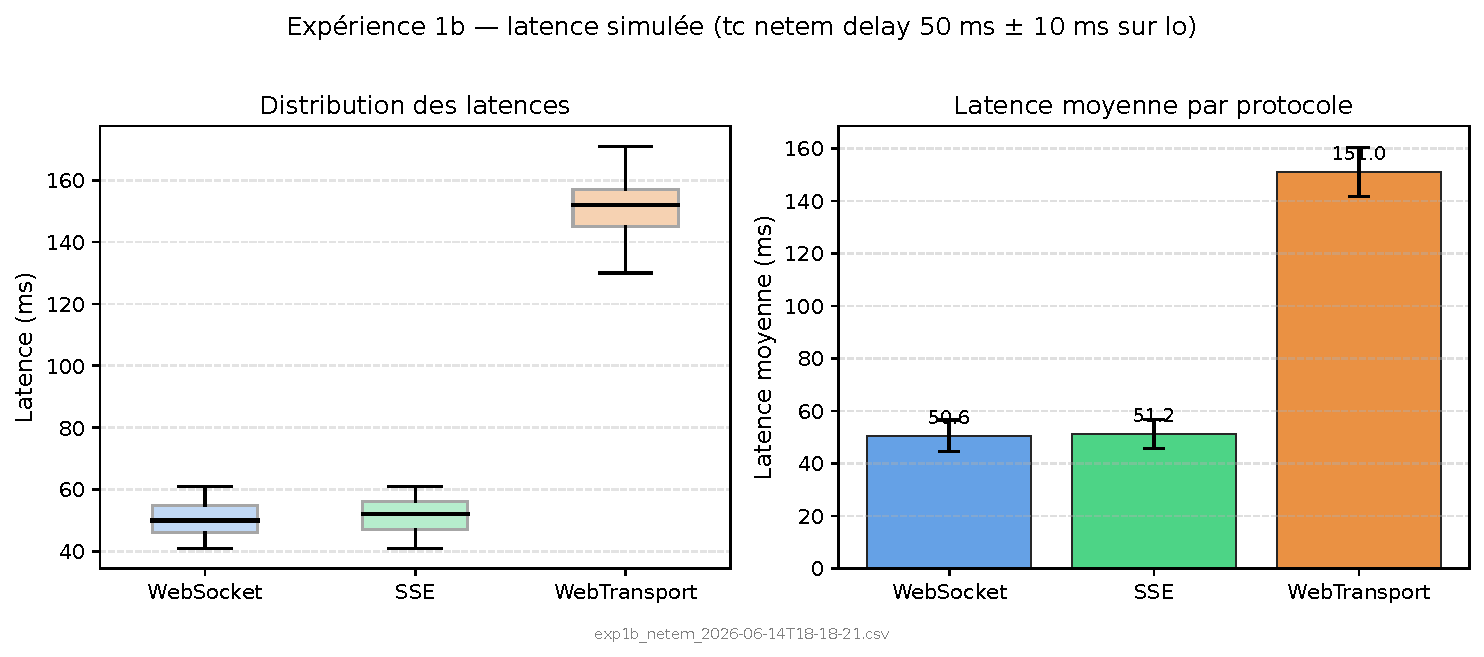
\includegraphics[width=0.85\textwidth]{articles/fig/exp1b_netem.pdf}
\caption{Expérience 1b --- latence simulée (\texttt{tc netem delay 50ms 10ms} sur \texttt{lo}). WebSocket et SSE $\sim$51 ms ; WebTransport $\sim$151 ms. À gauche : distribution des latences par protocole ; à droite : latence moyenne. Mesure complémentaire, conditions non symétriques entre interfaces.}
\end{figure}

\subsection{Expérience 2 --- Latence sous charge croissante}

Cette expérience fait varier la fréquence d'envoi de 1 à 100 messages par seconde, avec une mesure d'une minute par palier, afin d'observer si les protocoles se différencient lorsque le volume de données augmente et à partir de quel seuil.

\begin{table}[H]
\centering
\begin{tabular}{|l|c|c|c|}
\hline
\textbf{Fréquence} & \textbf{WebSocket (ms)} & \textbf{SSE (ms)} & \textbf{WebTransport (ms)} \\
\hline
1 msg/s & 0,35 & 0,24 & 0,30 \\
10 msg/s & 0,39 & 0,39 & 0,46 \\
50 msg/s & 0,30 & 0,35 & 0,51 \\
100 msg/s & 0,28 & 0,31 & 0,39 \\
\hline
\end{tabular}
\caption{Latence moyenne par fréquence (ms)}
\end{table}

\begin{table}[H]
\centering
\begin{tabular}{|l|c|c|c|c|}
\hline
\textbf{Fréquence cible} & \textbf{WebSocket} & \textbf{SSE} & \textbf{WebTransport} & \textbf{\% atteint} \\
\hline
1 msg/s & 1,01 & 1,01 & 1,01 & 101\% \\
10 msg/s & 9,98 & 9,98 & 9,97 & $\sim$100\% \\
50 msg/s & 49,46 & 49,44 & 49,46 & 99\% \\
100 msg/s & 98,48 & 98,37 & 98,15 & 98\% \\
\hline
\end{tabular}
\caption{Débit reçu par fréquence (msg/s)}
\end{table}

\begin{figure}[H]
\centering

\includegraphics[width=\textwidth]{articles/fig/exp2_charge.pdf}
\caption{Expérience 2 --- latence moyenne et débit reçu sous charge croissante (1 à 100 msg/s).}
\end{figure}

Les trois protocoles suivent la charge cible sur tous les paliers, atteignant entre 98\% et 101\% du débit visé, y compris à 100 messages par seconde. Aucun protocole ne perd de messages de façon significative : la légère perte de $\sim$2\% à 100 msg/s est négligeable et commune aux trois protocoles. Les latences moyennes restent inférieures à 1 ms sur l'ensemble des paliers testés. WebTransport affiche systématiquement la latence moyenne la plus élevée à partir de 10 msg/s, avec un écart de +0,07 à +0,21 ms selon le palier par rapport à WebSocket. Cet écart est modeste mais cohérent et reproductible sur tous les runs, ce qui suggère un surcoût de traitement lié au polyfill utilisé. Pour rappel, le polyfill est une bibliothèque logicielle qui émule WebTransport par-dessus WebSocket, faute de support natif stable dans Node.js. À 100 msg/s, WebSocket descend à 0,28 ms de latence moyenne. Cette légère amélioration par rapport aux paliers inférieurs s'explique probablement par le traitement en lot des messages TCP : à haute fréquence, plusieurs messages sont regroupés dans le même paquet réseau, ce qui réduit le coût moyen par message. Aucun protocole ne montre de dégradation brutale de la latence avec la montée en charge. Cela s'explique par le fait que les tests ont été réalisés en local sur la même machine : le facteur limitant n'est donc pas le protocole lui-même, mais simplement les performances de l'environnement de test.

\subsection{Expérience 3 --- Résilience face à une coupure réseau}

Cette expérience a été répétée 3 fois dans les mêmes conditions : les trois protocoles connectés simultanément à 1 msg/s, avec la reconnexion automatique activée dans le dashboard.

Pour simuler la coupure, on a utilisé un script basé sur \texttt{iptables}, un outil Linux qui fonctionne comme un pare-feu programmable permettant de bloquer ou d'autoriser le trafic réseau selon des règles précises. Concrètement, le script ajoute temporairement une règle qui bloque tout le trafic entrant et sortant sur les ports des trois serveurs (3001 pour WebSocket, 3002 pour SSE, 3003 pour WebTransport), puis supprime cette règle au bout de 5 secondes. Du point de vue des protocoles, cette interruption est indiscernable d'une vraie coupure réseau.

\begin{table}[H]
\centering
\small
\begin{tabular}{|l|c|c|c|l|}
\hline
\textbf{Run} & \textbf{WebSocket (ms)} & \textbf{SSE (ms)} & \textbf{WebTransport (ms)} & \textbf{Notes UI} \\
\hline
1 & 3065 & 2058 & 3066 & SSE repasse bleu en premier \\
2 & 2880 & 2070 & 2884 & idem \\
3 & 5400 & 2053 & 4444 & WS/WT plus lents \\
\textbf{Moyenne} & \textbf{3782} & \textbf{2060} & \textbf{3465} & \\
\hline
\end{tabular}
\caption{Temps de reconnexion après coupure réseau de 5 s (n=3 runs)}
\end{table}

\begin{figure}[H]
\centering

\includegraphics[width=0.6\textwidth]{articles/fig/exp3_reconnexion.pdf}
\caption{Expérience 3 --- temps de reconnexion moyen après coupure réseau de 5 s (n=3 runs).}
\end{figure}

SSE présente le temps de reconnexion le plus court et le plus stable sur les 3 runs, avec une moyenne de $\sim$2,06 s et un écart de moins de 20 ms entre les trois runs. Ce résultat s'explique par le fait que SSE bénéficie d'une reconnexion native gérée directement par le navigateur en passant par l'API \texttt{EventSource} : dès que la connexion est perdue, le navigateur tente automatiquement de se reconnecter sans qu'aucune ligne de code supplémentaire ne soit nécessaire côté application. SSE est également le premier protocole à repasser en état « Connecté » dans le dashboard à chaque run.

WebSocket et WebTransport affichent des temps plus élevés et plus variables, avec une moyenne de 3,78 s pour WebSocket et 3,46 s pour WebTransport. Ces deux protocoles ne bénéficient pas de reconnexion native : c'est le code applicatif qui détecte la déconnexion et tente de se reconnecter toutes les secondes. Le run 3 montre un pic à 5,4 s pour WebSocket. Ce pic s'explique par le fait qu'une reconnexion gérée manuellement n'est pas précise : selon le moment où le code détecte la coupure et tente de se reconnecter, le délai peut varier d'un run à l'autre.

\paragraph{Comportement UI pendant la coupure.}
Pendant la coupure, les trois protocoles se comportent de façon similaire côté interface : les graphiques se figent car plus aucune donnée n'arrive, et les pastilles passent en orange pour indiquer la perte de connexion. La différence se joue uniquement sur la vitesse de reprise après le rétablissement du réseau, SSE reprenant toujours en premier.

\begin{table}[H]
\centering
\small
\begin{tabular}{|l|p{4.5cm}|p{5cm}|}
\hline
\textbf{Protocole} & \textbf{Pendant la coupure} & \textbf{Après rétablissement réseau} \\
\hline
WebSocket & Graphique figé, pastille orange « Reconnexion… » & Pastille bleue « Reconnecté » ($\sim$3--5 s), puis flux repris \\
\hline
SSE & Graphique figé, pastille orange brève & \textbf{Premier} en bleu ($\sim$2 s), reprise la plus rapide visuellement \\
\hline
WebTransport & Graphique figé, pastille orange & Bleu après WS et SSE ($\sim$3--4 s en moyenne) \\
\hline
\end{tabular}
\caption{Comportement de l'interface pendant et après la coupure réseau}
\end{table}

\subsection{Expérience 4 --- Complexité d'intégration}

L'évaluation repose sur une grille de cinq critères, chacun noté de 1 (très facile) à 5 (très difficile), pour un score maximum de 25 points. Cette approche structurée évite un jugement global subjectif : chaque note est justifiée par un élément concret du code ou du processus de mise en place. Les cinq critères évalués sont :

\begin{itemize}
    \item \textbf{Mise en place serveur :} facilité de démarrage et de configuration du serveur ;
    \item \textbf{API client :} simplicité de la connexion et de la réception des données côté Angular ;
    \item \textbf{Gestion reconnexion :} effort nécessaire pour gérer les déconnexions et reconnexions ;
    \item \textbf{Débogage et clarté des erreurs :} facilité à identifier et corriger les problèmes ;
    \item \textbf{Documentation et écosystème :} richesse des ressources disponibles (exemples, bibliothèques, support).
\end{itemize}

\begin{table}[H]
\centering
\begin{tabular}{|l|c|c|c|}
\hline
\textbf{Critère} & \textbf{WebSocket} & \textbf{SSE} & \textbf{WebTransport} \\
\hline
Mise en place serveur & 1 & 2 & 5 \\
API client & 2 & 1 & 4 \\
Gestion reconnexion & 3 & 1 & 3 \\
Débogage et clarté des erreurs & 2 & 2 & 5 \\
Documentation et écosystème & 2 & 2 & 4 \\
\hline
\textbf{Total /25} & \textbf{10} & \textbf{8} & \textbf{21} \\
\hline
\end{tabular}
\caption{Grille de complexité d'intégration (1 = très facile, 5 = très difficile)}
\end{table}

SSE obtient le score le plus bas (8/25), ce qui en fait le protocole le plus simple à intégrer. Son serveur ne nécessite qu'Express et CORS, deux bibliothèques légères ; son API client se résume à \texttt{new EventSource(url)} en une ligne et sa reconnexion est native. WebSocket reste accessible (10/25) : son serveur ne requiert qu'une seule dépendance (\texttt{ws}), mais la reconnexion doit être codée manuellement côté client.

WebTransport cumule les difficultés sur quasiment tous les critères (21/25). Côté serveur, il a fallu générer un certificat SSL autosigné, configurer le serveur pour écouter sur l'IP du réseau local (et non juste \texttt{localhost}), et installer un polyfill. Côté navigateur, Chrome devait être lancé avec des flags spéciaux pour accepter le certificat. Les erreurs rencontrées lors de la mise en place étaient souvent peu explicites, rendant le débogage particulièrement difficile. Ces difficultés corroborent les résultats de l'expérience 3 : le surcoût de configuration de WebTransport ne se traduit pas par un gain de performance notable dans notre contexte local.

Le détail des notes, justifiées par des éléments concrets du code et de la mise en place, est présenté ci-dessous :

\begin{table}[H]
\centering
\footnotesize
\begin{tabular}{|p{2cm}|c|c|c|p{8cm}|}
\hline
\textbf{Critère} & \textbf{WS} & \textbf{SSE} & \textbf{WT} & \textbf{Justification (extraits code / setup)} \\
\hline
Mise en place serveur & 1 & 2 & 5 & WS : \texttt{websocket-server.js} ($\sim$20 L), bibliothèque \texttt{ws} seule. SSE : Express + CORS + routes (\texttt{sse-server.js}, $\sim$62 L). WT : \texttt{cert.pem}/\texttt{key.pem}, \texttt{npm run setup:wt}, scripts de génération de certificat, écoute sur \texttt{0.0.0.0:3003}. \\
\hline
API client & 2 & 1 & 4 & SSE : \texttt{new EventSource(url)} + handlers. WS : \texttt{new WebSocket(url)} + $\sim$60 L. WT : polyfill \texttt{@fails-components/}\allowbreak\texttt{webtransport}, hash SPKI, boucle \texttt{datagrams.readable} ($\sim$120 L). \\
\hline
Gestion reconnexion & 3 & 1 & 3 & SSE : reconnexion native \texttt{EventSource} ($\sim$2,06 s, stable). WS / WT : timer 1 s + détection de messages bloqués (pas de reconnexion native). \\
\hline
Débogage / erreurs & 2 & 2 & 5 & WS : \texttt{onclose} explicite. SSE : \texttt{onerror} peu détaillé. WT : échecs de handshake / certificat, lancement de Chrome avec flags, IP LAN requise. \\
\hline
Documentation / écosystème & 2 & 2 & 4 & WS et SSE : MDN + bibliothèques Node matures. WT : draft / polyfill, peu d'exemples correspondant à une stack WSL identique. \\
\hline
\textbf{Total /25} & \textbf{10} & \textbf{8} & \textbf{21} & \\
\hline
\end{tabular}
\caption{Détail des notes de complexité d'intégration et justifications}
\end{table}

% --------------------------------------------------
\section{Discussion}
% --------------------------------------------------

\subsection{Latence : des différences faibles mais cohérentes}

Les quatre expériences montrent que, dans un environnement local, les trois protocoles transmettent des données en temps réel avec des latences très faibles (inférieures à 1 ms en moyenne). À ce niveau, les différences sont difficiles à percevoir à l'œil nu dans une vraie interface utilisateur.

Cependant, certaines tendances ressortent de façon cohérente : WebSocket affiche la latence moyenne la plus faible à haute fréquence (0,28 ms à 100 msg/s) --- c'est le protocole le plus mature et le plus optimisé pour ce type d'usage ; SSE se comporte de façon très proche de WebSocket, avec un léger surcoût lié au format texte imposé par le standard et au parsing HTTP supplémentaire ; WebTransport affiche systématiquement une latence légèrement plus élevée, probablement due au polyfill plutôt qu'à QUIC lui-même. On ne peut donc pas conclure que WebTransport est intrinsèquement plus lent --- dans un environnement de production avec support natif complet, les résultats pourraient être différents.

Le pic isolé à 43 ms sur WebTransport confirme que l'établissement initial de la connexion QUIC est plus coûteux que pour TCP. Ce délai ponctuel peut avoir un impact perceptible si l'application se reconnecte fréquemment.

\subsection{Débit : les trois protocoles sont équivalents}

L'expérience 2 montre que les trois protocoles atteignent 98 à 101\% du débit cible sur tous les paliers testés, jusqu'à 100 messages par seconde. Dans notre contexte local, aucun protocole ne présente de perte de messages significative. Cette équivalence de débit est un résultat important : elle montre que le choix du protocole n'a pas d'impact sur la capacité à transmettre un volume élevé de données dans des conditions normales.

\subsection{Résilience : l'avantage clair de SSE}

L'expérience 3 révèle la différence la plus marquante. SSE se reconnecte en moyenne en 2,06 s, de façon stable et reproductible sur les 3 runs. WebSocket et WebTransport mettent en moyenne 3,78 s et 3,46 s respectivement, avec une variabilité plus importante.

Cet écart s'explique par une différence fondamentale de conception : SSE bénéficie d'une reconnexion native gérée directement par le navigateur grâce à l'API \texttt{EventSource}, sans qu'aucun code supplémentaire ne soit nécessaire. WebSocket et WebTransport, eux, nécessitent une logique de reconnexion codée manuellement côté client, ce qui introduit un délai de détection avant chaque tentative de reconnexion. Pour une IHM destinée à afficher des données critiques en temps réel (comme un tableau de bord de monitoring), cette différence de $\sim$1,7 seconde peut avoir un impact réel sur l'expérience utilisateur.

\subsection{Complexité d'intégration : un facteur décisif}

Les écarts entre protocoles sont importants en termes d'effort de développement. SSE (8/25) et WebSocket (10/25) restent accessibles et bien documentés. WebTransport (21/25) cumule en revanche de nombreuses difficultés : génération de certificat SSL, configuration spécifique du navigateur, utilisation d'un polyfill, messages d'erreur peu clairs lors du débogage. Ce surcoût de mise en place est d'autant plus difficile à justifier que les gains de performance de WebTransport restent faibles dans notre configuration. En production, sur un vrai réseau avec de la latence et des pertes de paquets, les avantages de QUIC pourraient devenir plus significatifs, mais cela reste à vérifier dans un contexte réel.

\subsection{Réponse à la problématique}

Notre problématique était la suivante :

\begin{center}
\textit{Dans quelle mesure le choix du protocole de communication temps réel influence-t-il les performances et l'expérience utilisateur d'un dashboard Angular, et quel protocole offre le meilleur compromis entre latence, résilience et complexité d'intégration ?}
\end{center}

Les expérimentations menées permettent d'apporter les éléments de réponse suivants :

En conditions locales, le choix du protocole a un impact limité sur la latence et le débit. Les trois protocoles sont capables de transmettre des données en temps réel de façon efficace. La différence devient plus perceptible sur la résilience (SSE se reconnecte plus vite et de façon plus stable) et sur la complexité d'intégration (WebTransport est nettement plus difficile à mettre en place).

Si l'on cherche le meilleur compromis global pour une IHM Angular en 2025, SSE apparaît comme le choix le plus équilibré pour un cas d'usage de push serveur simple : latence faible, reconnexion native, code minimal, documentation abondante. WebSocket reste pertinent dès que la bidirectionnalité est nécessaire, par exemple pour une application où le client doit aussi envoyer des données au serveur. WebTransport est prometteur mais sa complexité d'intégration actuelle et son support encore partiel le réservent à des cas d'usage très spécifiques nécessitant des performances réseau extrêmes.

\subsection{Limites de l'étude}

Plusieurs limites doivent être prises en compte pour nuancer ces conclusions :

\begin{itemize}
    \item \textbf{Environnement local uniquement :} toutes les mesures ont été réalisées sur une même machine en \texttt{localhost}. Les latences obtenues (< 1 ms) ne sont pas représentatives d'un environnement de production réel où le réseau introduit des délais bien plus importants. Les avantages théoriques de QUIC, notamment sa meilleure résistance aux pertes de paquets, n'ont pas pu être observés dans ces conditions.
    \item \textbf{Synchronisation des horloges :} la latence est mesurée comme la différence entre le \texttt{timestamp} émis par le serveur (Node sous WSL2/Linux) et l'heure de réception côté navigateur (Chrome sous Windows). Cette mesure \textit{one-way} suppose que les deux horloges sont alignées --- ce qui est le cas en pratique car WSL2 se cale sur l'horloge de l'hôte Windows, et ce que confirment les faibles latences mesurées. Une approche plus rigoureuse reposerait sur un aller-retour (RTT/2) avec une horloge unique.
    \item \textbf{WebTransport avec polyfill :} l'implémentation de WebTransport utilisée dans ce projet repose sur un polyfill qui émule le protocole par-dessus WebSocket, et non sur une implémentation native de QUIC. Les performances mesurées pour WebTransport ne reflètent donc pas nécessairement ce qu'on observerait avec un support natif complet dans le navigateur et le serveur.
    \item \textbf{Support navigateur limité :} WebTransport n'était pas supporté par Firefox au moment de cette étude. Nous avons donc utilisé Chrome pour tous les tests. Dans un contexte de production, cette contrainte de compatibilité est un facteur important à prendre en compte.
    \item \textbf{Nombre de runs limité :} l'expérience 3 n'a été répétée que 3 fois par manque de temps. Un nombre plus élevé de runs permettrait d'obtenir des moyennes plus fiables et de mieux caractériser la variabilité des temps de reconnexion.
    \item \textbf{Cas d'usage unique :} les expériences ont été réalisées sur un seul type d'application : un dashboard de données simulées. D'autres cas d'usage (jeu en ligne, outil collaboratif, streaming vidéo) pourraient donner des résultats très différents.
\end{itemize}

% --------------------------------------------------
\section{Conclusion}
% --------------------------------------------------

\subsection{Synthèse des travaux}

Ce projet avait pour objectif de comparer trois protocoles de communication temps réel --- WebSocket, Server-Sent Events et WebTransport --- dans le contexte du développement d'une IHM web Angular. Pour y répondre, nous avons développé un banc de test complet composé d'un backend Node.js exposant trois serveurs distincts et d'un dashboard Angular mesurant les performances en temps réel. Quatre expériences ont été menées : latence en conditions normales, latence sous charge croissante, résilience face à une coupure réseau et complexité d'intégration.

\subsection{Principaux apports}

Les résultats obtenus permettent de tirer plusieurs conclusions concrètes :

\textbf{Sur la latence et le débit}, les trois protocoles sont équivalents dans un environnement local. Les latences moyennes restent toutes inférieures à 1 ms et le débit atteint 98 à 101\% de la cible jusqu'à 100 messages par seconde. Dans ces conditions, le choix du protocole n'a pas d'impact perceptible sur la fluidité de l'interface.

\textbf{Sur la résilience}, SSE se démarque nettement grâce à sa reconnexion native gérée par le navigateur ($\sim$2,06 s en moyenne), contre $\sim$3,5 à 3,8 s pour WebSocket et WebTransport qui nécessitent une reconnexion codée manuellement. Pour une IHM affichant des données critiques, cette différence peut avoir un impact réel sur l'expérience utilisateur.

\textbf{Sur la complexité d'intégration}, SSE est le protocole le plus simple à mettre en place (8/25), suivi de WebSocket (10/25). WebTransport cumule de nombreuses difficultés de configuration (21/25) : certificat SSL, flags navigateur, polyfill, pour un gain de performance limité dans notre contexte.

\subsection{Recommandations pratiques}

À l'issue de ce travail, on peut formuler les recommandations suivantes pour un développeur d'IHM web confronté à ce choix :

\begin{itemize}
    \item \textbf{Choisir SSE} pour un cas d'usage de push serveur simple (dashboard, notifications, flux de données unidirectionnel) : c'est le protocole le plus simple, le plus résilient et le mieux supporté.
    \item \textbf{Choisir WebSocket} dès que la communication bidirectionnelle est nécessaire (chat, jeu en ligne, outil collaboratif) : c'est le standard mature pour ce type d'usage.
    \item \textbf{Attendre WebTransport} pour des cas d'usage nécessitant des performances réseau extrêmes sur des réseaux instables. Le protocole est prometteur mais son support natif reste encore trop limité en 2025 pour une utilisation en production sereine.
\end{itemize}

\subsection{Perspectives}

Ce travail ouvre plusieurs pistes d'approfondissement qui n'ont pas pu être explorées dans le cadre de ce projet :

\begin{itemize}
    \item Reproduire les expériences sur un vrai réseau, avec de la latence et des pertes de paquets réelles, pour mieux observer les avantages théoriques de QUIC face à TCP.
    \item Tester WebTransport avec un support natif complet (sans polyfill), lorsque les navigateurs et les bibliothèques serveur auront atteint une maturité suffisante : les résultats pourraient être significativement différents.
    \item Étendre les expériences à d'autres cas d'usage comme la communication bidirectionnelle ou le streaming de données binaires, pour lesquels WebTransport pourrait montrer des avantages plus marqués.
    \item Mesurer l'impact côté serveur en termes de consommation CPU et mémoire lors de connexions simultanées nombreuses, que notre banc de test ne couvrait pas.
\end{itemize}

Ce travail m'a permis de combiner deux domaines qui m'intéressent, les réseaux et le développement web, en explorant une question concrète que tout développeur d'IHM est amené à se poser. Il m'a aussi montré que WebTransport, bien que prometteur sur le papier, reste encore difficile à exploiter en pratique, et que des technologies plus simples comme SSE peuvent parfois être le meilleur choix malgré leur apparente modestie technique.

% --------------------------------------------------
\section{Références}
% --------------------------------------------------

\subsection*{Standards et spécifications officielles}

\begin{itemize}
    \item IETF. \textit{RFC 6455 --- The WebSocket Protocol}. 2011. \url{https://datatracker.ietf.org/doc/html/rfc6455}
    \item IETF. \textit{RFC 8441 --- Bootstrapping WebSockets with HTTP/2}. 2018. \url{https://datatracker.ietf.org/doc/html/rfc8441}
    \item IETF. \textit{RFC 9000 --- QUIC: A UDP-Based Multiplexed and Secure Transport}. 2021. \url{https://datatracker.ietf.org/doc/html/rfc9000}
    \item IETF. \textit{RFC 9114 --- HTTP/3}. 2022. \url{https://datatracker.ietf.org/doc/html/rfc9114}
    \item W3C. \textit{Server-Sent Events}. 2015. \url{https://www.w3.org/TR/eventsource/}
    \item W3C / IETF. \textit{WebTransport --- Working Draft}. 2024. \url{https://www.w3.org/TR/webtransport/}
\end{itemize}

\subsection*{Documentation technique officielle}

\begin{itemize}
    \item MDN. \textit{WebSocket API}. \url{https://developer.mozilla.org/en-US/docs/Web/API/WebSockets_API}
    \item MDN. \textit{Server-Sent Events}. \url{https://developer.mozilla.org/en-US/docs/Web/API/Server-sent_events}
    \item MDN. \textit{WebTransport API}. \url{https://developer.mozilla.org/en-US/docs/Web/API/WebTransport_API}
    \item MDN. \textit{WebTransport() constructor --- serverCertificateHashes}. \url{https://developer.mozilla.org/en-US/docs/Web/API/WebTransport/WebTransport}
    \item Google Chrome Developers. \textit{WebTransport explainer}. \url{https://developer.chrome.com/docs/capabilities/web-apis/webtransport}
    \item Google Chrome. \textit{WebTransport --- exemple officiel client}. \url{https://googlechrome.github.io/samples/webtransport/client.html}
    \item Google Chrome. \textit{Serveur de référence WebTransport (Python)}. \url{https://github.com/GoogleChrome/samples/blob/gh-pages/webtransport/webtransport_server.py}
    \item Chrome Platform Status. \textit{Statut WebTransport dans Chrome}. \url{https://www.chromestatus.com/feature/4854144902889472}
    \item Chromium Source. \textit{Restriction RSA pour serverCertificateHashes}. \url{https://chromium.googlesource.com/chromium/src/net/+/refs/heads/main/quic/dedicated_web_transport_http3_client.cc}
    \item Chromium. \textit{Lancer Chromium avec des flags}. \url{https://www.chromium.org/developers/how-tos/run-chromium-with-flags/}
\end{itemize}

\subsection*{Articles et comparaisons techniques}

\begin{itemize}
    \item Aptuz. \textit{WebSockets vs SSE vs WebTransport}. \url{https://aptuz.com/blog/websockets-vs-sse-vs-webtransports/}
    \item RxDB. \textit{WebSockets vs SSE vs Polling vs WebRTC vs WebTransport}. \url{https://rxdb.info/articles/websockets-sse-polling-webrtc-webtransport.html}
    \item Reddit / r/programming. \textit{WebSockets vs SSE vs Long Polling vs WebTransport}. 2024. \url{https://www.reddit.com/r/programming/comments/1bhqrhp/websockets_vs_serversentevents_vs_longpolling_vs/}
\end{itemize}

\subsection*{Résolution de problèmes (Stack Overflow)}

\begin{itemize}
    \item Stack Overflow. \textit{Certificat auto-signé et ECDSA pour WebTransport}. \url{https://stackoverflow.com/questions/75979276}
    \item Stack Overflow. \textit{Opening handshake failed avec WebTransport en local}. \url{https://stackoverflow.com/questions/77447254}
\end{itemize}

\subsection*{Bibliothèques et outils utilisés}

\begin{itemize}
    \item \texttt{ws} --- WebSocket library for Node.js. \url{https://github.com/websockets/ws}
    \item \texttt{@fails-components/webtransport} --- WebTransport polyfill. \url{https://github.com/fails-components/webtransport}
    \item \texttt{webtransport-go} --- implémentation WebTransport en Go. \url{https://github.com/adriancable/webtransport-go}
    \item Angular. \url{https://angular.dev}
    \item Node.js. \url{https://nodejs.org}
    \item Express. \url{https://expressjs.com}
\end{itemize}

\subsection*{Outils réseau}

\begin{itemize}
    \item Linux man pages. \textit{iptables}. \url{https://man7.org/linux/man-pages/man8/iptables.8.html}
    \item Linux man pages. \textit{tc --- traffic control}. \url{https://man7.org/linux/man-pages/man8/tc.8.html}
\end{itemize}
